\documentclass[aspectratio=169]{beamer} % 16:9 aspect ratio for modern screen
% \documentclass[handout]{beamer}
% \documentclass[notes=only]{beamer}

% Theme settings
\usetheme[progressbar=foot]{metropolis} % Minimalist theme
\metroset{progressbar=frametitle} % Progress bar soll nur folien mit titel berücksichtigtigen?
\setbeamercolor{background canvas}{bg=white} % White background color

\makeatletter
    \setlength{\metropolis@progressinheadfoot@linewidth}{1.5pt}
\makeatother


\usefonttheme{professionalfonts} % Font theme

% Packages
\usepackage[T1]{fontenc}   % Font encoding
\usepackage[ngerman]{babel} % German language
\usepackage[sfdefault]{FiraSans} % For FiraSans font
\usepackage[backend=biber, style=authoryear-comp
, sorting=nyt]{biblatex} % For bibliography
\usepackage{csquotes} % Recommended for biblatex with babel/polyglossia
\usepackage{textgreek} % Greek letters in text mode (aus references von Citavi)
\usepackage{tikz}          % For drawing graphics
\usepackage{animate} % Für Animation

\usepackage{graphicx}       % For including images
\usepackage{amsmath, amssymb} % For math symbol

% \usepackage{media9} % For embedding videos

\usepackage[labelformat=empty]{caption}


% Bibliography settings
\addbibresource{references.bib} % Path to the bibliography file

% Graphics path
\graphicspath{{Images/}} % Path to images folder

% custom Citation commands
\DeclareCiteCommand{\citeauthortitle}
  {\usebibmacro{prenote}}
  {\usebibmacro{citeindex}%
   \printnames{labelname}%
   \setunit{\space\textendash\space}
   \printfield{title}}
  {\multicitedelim}
  {\usebibmacro{postnote}}

  \DeclareCiteCommand{\citeauthortitleurl}
  {\usebibmacro{prenote}}
  {\usebibmacro{citeindex}%
   \printnames{labelname}%
   \setunit{\space\textendash\space}
   \printfield{title}%
   \setunit{\addsemicolon\space}
   \printfield{url}}
  {\multicitedelim}
  {\usebibmacro{postnote}}

\DeclareCiteCommand{\parenciteauthortitle}
  {\usebibmacro{prenote}}
  {\bibopenparen\usebibmacro{citeindex}%
   \printnames{labelname}%
   \setunit{\space\textendash\space}% <- Hier wird das Trennzeichen ":" hinzugefügt
   \printfield{title}\bibcloseparen}
  {\multicitedelim}
  {\usebibmacro{postnote}}

\makeatletter
\renewcommand\footnotesize{\tiny}
\makeatother

\newcommand{\figcite}[1]{\\[-3mm]{\tiny Quelle: \cite{#1}}}
\newcommand{\figciteweb}[1]{\\[-3mm]{\tiny aus: \citeauthortitle{#1}}}
\newcommand{\figciteweburl}[1]{\\[-3mm]{\tiny aus: \citeauthortitleurl{#1}}}
  
\mode<handout>{
    \AtBeginSection[]{} % In Handout-Version keine Section-Folie erzeugen
}

% Title page settings
\title{Interactions of Charged Particles with Matter}
\subtitle{Themavergabe und Betreuer: \textbf{Dr. Roman Bergert}}
\author{Florian Marius Adamczyk}
\date{\today}
\institute{Justus-Liebig-Universität Gießen \\ Modul \textbf{Wissenschaftliches Präsentieren} bei \textbf{Prof. Dr. Derck Schlettwein, PD Dr. Daniel Ebeling, Dr. Ulrike Nespital}\\ }
\titlegraphic{\vspace{-1cm}
\includegraphics[height=1.2cm]{Images/jlu_logo.jpg}}

\begin{document}

    % Black slide
    \begin{frame}<handout:0>[plain, noframenumbering]
        \begin{tikzpicture}[remember picture, overlay]
          \fill[black] (current page.south west) rectangle (current page.north east);
        \end{tikzpicture}
        \pause
        \centering
       {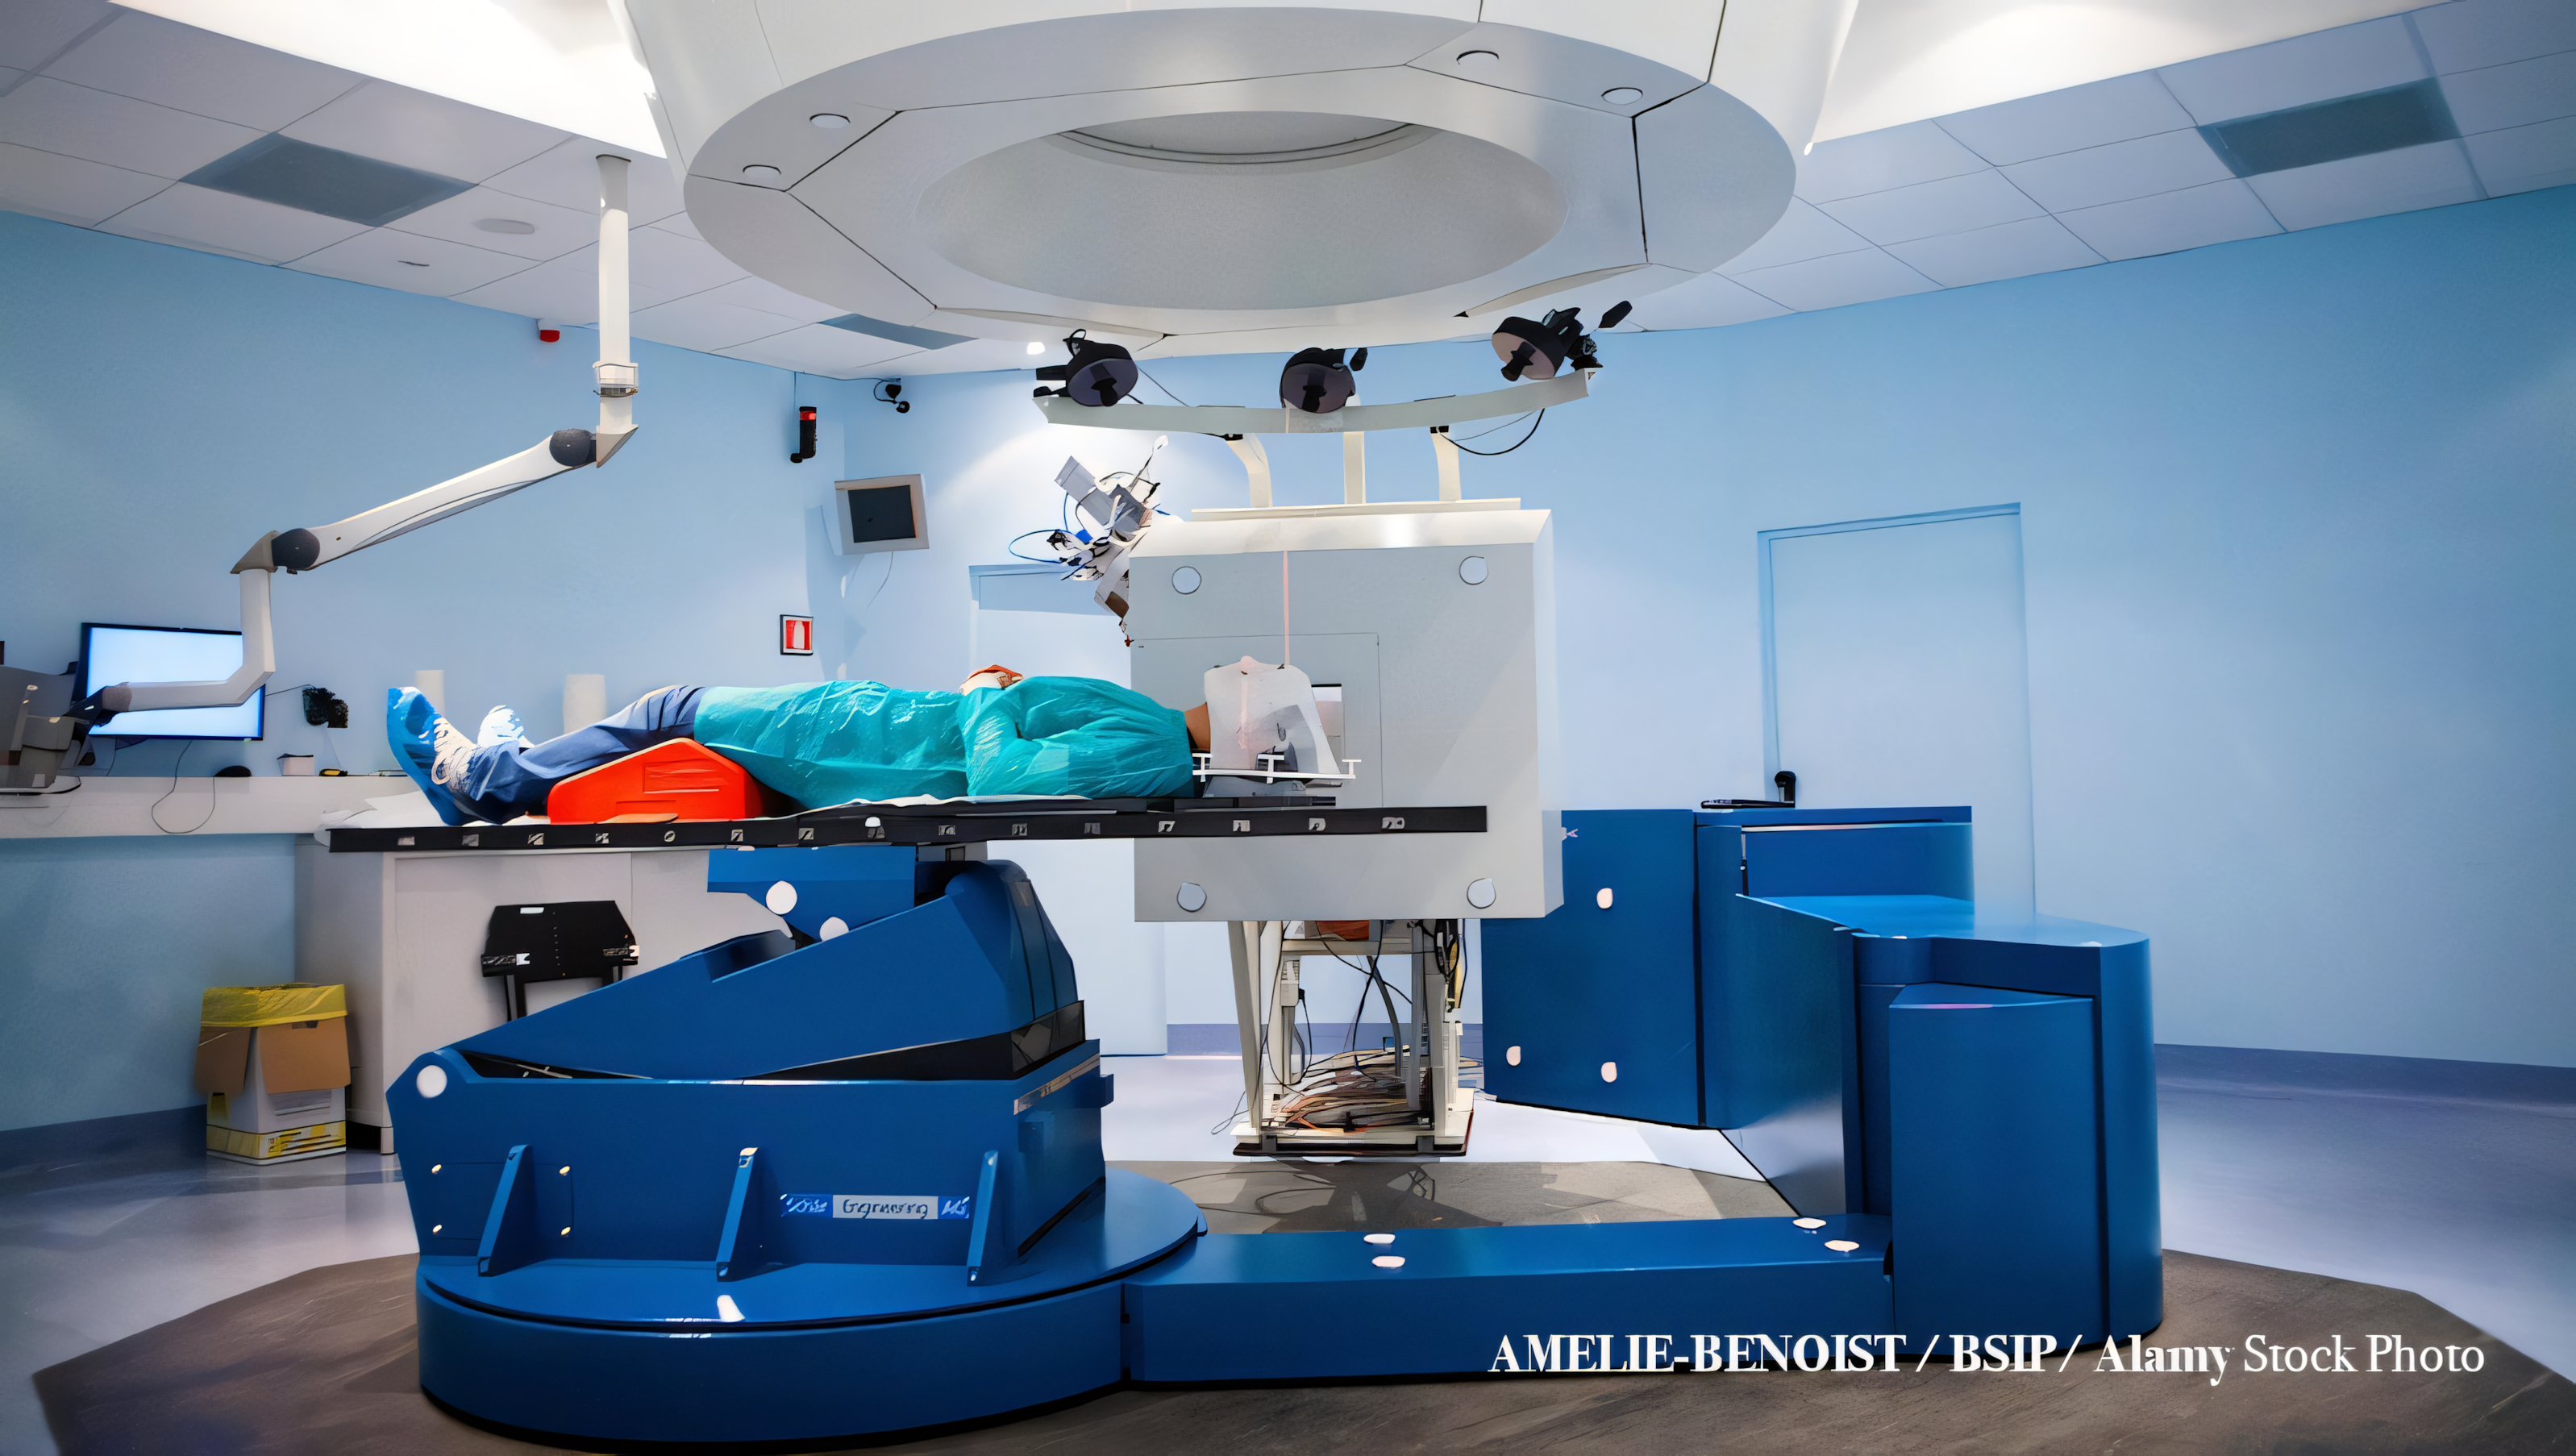
\includegraphics[width=0.9\textwidth]{Images/Titlepage.png}}
        \tiny \textcolor{gray}{aus: \cite{}  }
    \end{frame}
   

% Title Slide
\begin{frame}[noframenumbering, plain]
    \vspace*{-0.6cm}
    	itlepage
    \vspace*{-1.6cm}
\end{frame}

% Table of Contents
\begin{frame}<handout:0>{Gliederung}
    \setcounter{page}{1}
    	ableofcontents
    \note{Ich führe durch sechs Blöcke: Motivation, Bremsvermögen, Bethe-Formel, Bethe-Kurve, Bragg-Peak und eine Zusammenfassung.}
\end{frame}

% presentation slides %%%%%%%%%%%%%%%%%%%%%%%%%%%%%%%%%%%%%%%%%%%%%%%%%%%%%%%%%%%%%%%%%%

\section{Einleitung}
\begin{frame}[noframenumbering, plain]{Vielen Dank!}
        \vfill
        \centering
        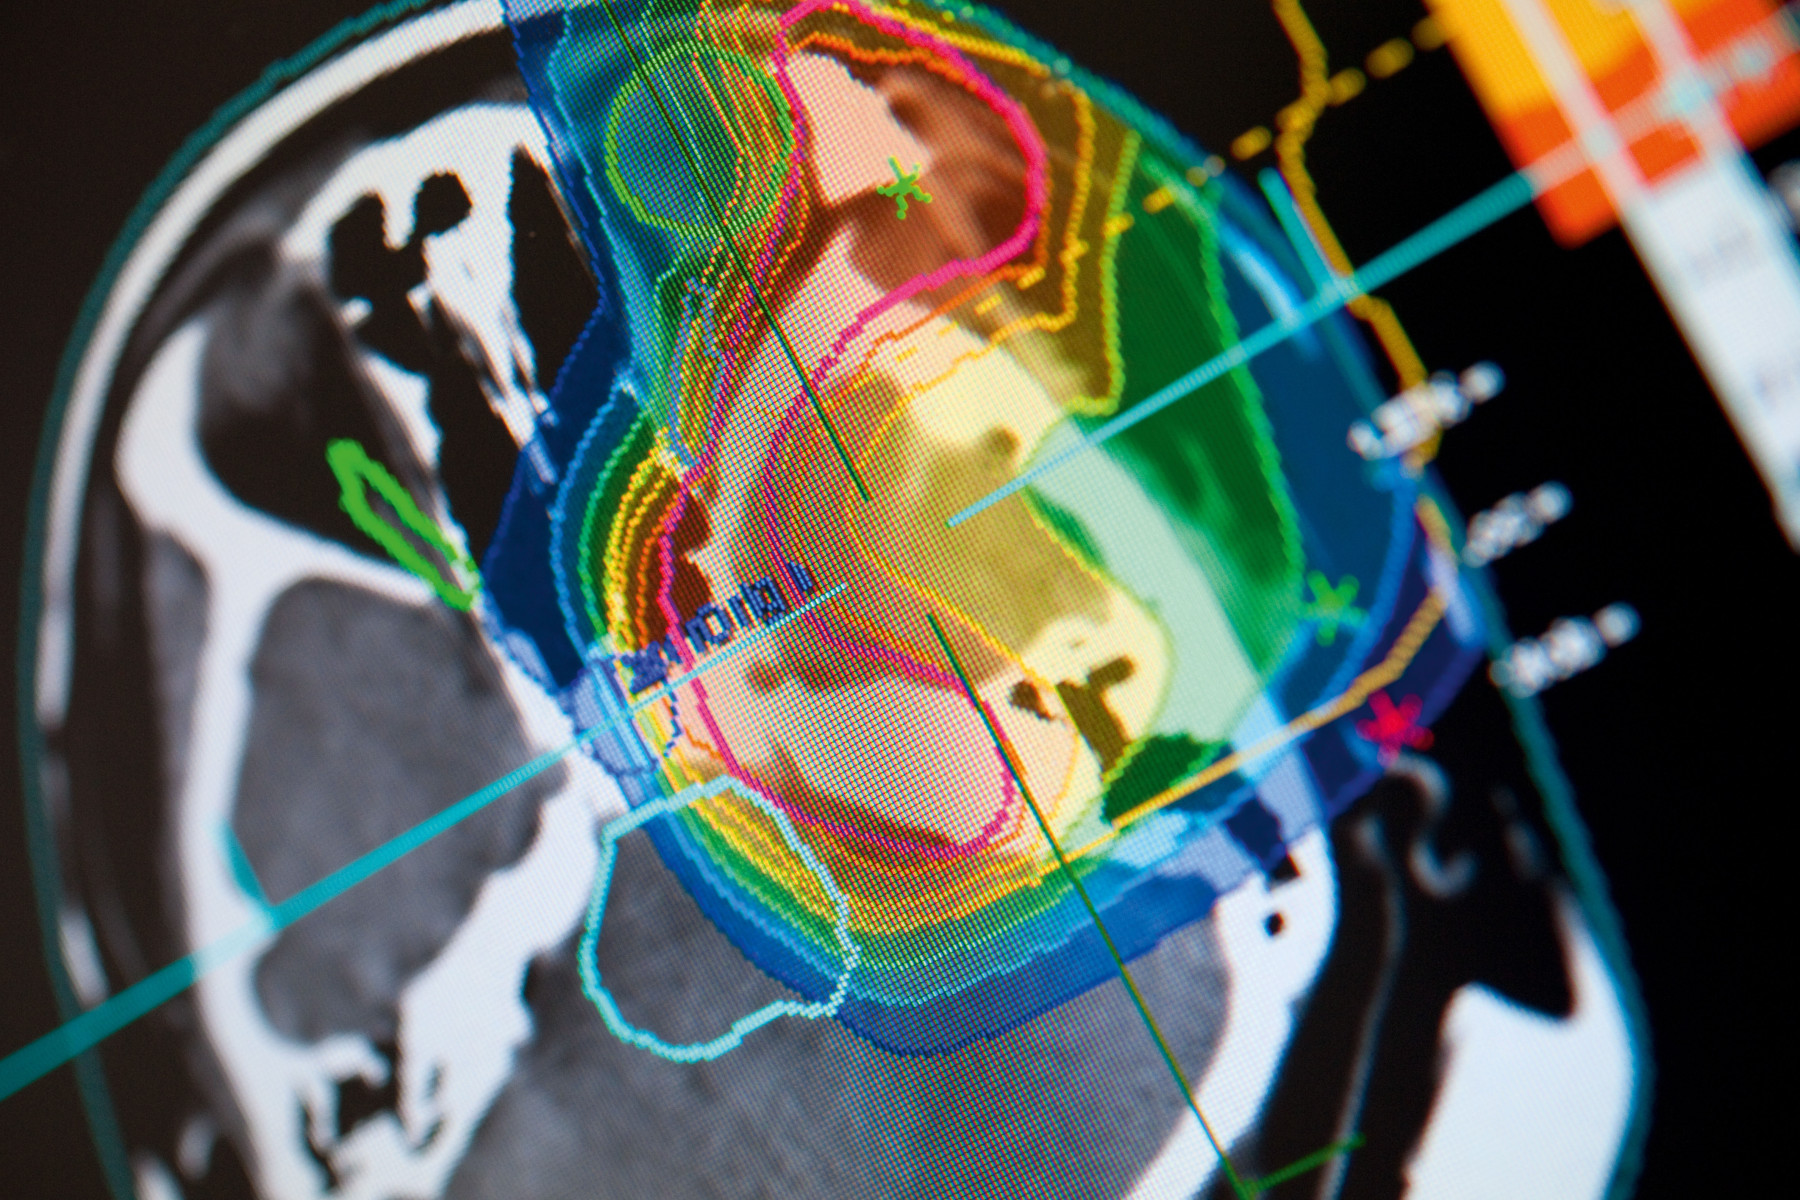
\includegraphics[width=0.8\textwidth]{1920_hirntumorbestrahlung.jpg}
        \figcite{HIT2019Image}
        \vfill
        \note{Ich danke für die Aufmerksamkeit und stehe nun für Fragen zur Verfügung.}
\end{frame}
                \item Korrekturen: Schalenkorrektur $C/Z$ und Dichteeffekt $\delta$.
            \end{itemize}
        \end{column}
        \begin{column}{0.48\textwidth}
            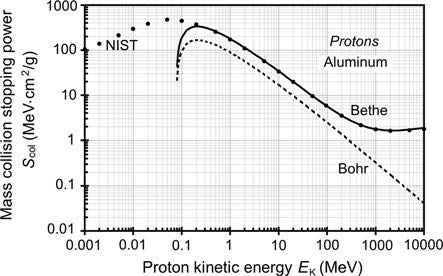
\includegraphics[width=\linewidth]{BetheKorr.jpeg}
            \figcite{Podgorsak2016}
        \end{column}
    \end{columns}
    \note{Die Bethe-Formel zeigt, dass die Bremskraft mit dem Quadrat der Projektileladung skaliert und im nichtrelativistischen Bereich umgekehrt proportional zur Geschwindigkeit ist. Die Elektronendichte des Absorbers und die mittlere Ionisationsenergie bestimmen die Materialabhängigkeit, wobei $Z/A$ für die meisten Elemente nahe 0,5 liegt \cite[S.\,246]{Podgorsak2016}. Relativistische Terme werden bei $\beta$ nahe 1 relevant und verursachen den langsamen Wiederanstieg der Bremskraft. Zur Anpassung an Messdaten werden die Schalenkorrektur bei niedrigen Energien und der Dichteeffekt bei hohen Energien berücksichtigt.}
\end{frame}

\section{Bethe-Kurve}
\begin{frame}{Form der Bethe-Kurve}
    \begin{columns}[T,totalwidth=\textwidth]
        \begin{column}{0.48\textwidth}
            \begin{itemize}
                \item Region 1: Anstieg bis zum Maximum bei etwa $250\,I$.
                \item Region 2: $1/\beta^{2}$-Abfall zur Minimum-Ionizing-Particle-Region.
                \item Region 3: Relativistischer Wiederanstieg, durch Dichteeffekt gedämpft.
            \end{itemize}
        \end{column}
        \begin{column}{0.48\textwidth}
            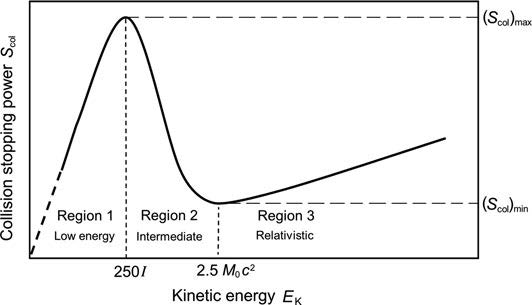
\includegraphics[width=\linewidth]{BetheCurve.jpeg}
            \figcite{Podgorsak2016}
        \end{column}
    \end{columns}
    \note{Die Auftragung des Kollisionsbremsvermögens als Funktion der kinetischen Energie zeigt drei Regionen \cite[S.\,249]{Podgorsak2016}. In der Niedrigenergiezone steigt $S_{\text{col}}$ bis zu einem Maximum, wobei die klassische Theorie versagt und Schalenkorrekturen nötig sind. Im intermediären Bereich fällt $S_{\text{col}}$ proportional zu $1/\beta^{2}$ und erreicht ein breites Minimum, die MIP-Region, nahezu materialunabhängig bei etwa $2{,}5 M_{0} c^{2}$. Bei hohen Energien steigt $S_{\text{col}}$ langsam wieder an, was durch den Dichteeffekt kondensierter Medien abgeschwächt wird.}
\end{frame}

\section{Bragg-Peak}
\begin{frame}{Bragg-Peak: Energiedeposition}
    \begin{columns}[T,totalwidth=\textwidth]
        \begin{column}{0.52\textwidth}
            \begin{itemize}
                \item Kollisionsverluste dominieren schwere geladene Teilchen.
                \item $S_{\text{col}} \propto 1/\beta^{2}$ erzeugt einen späten Energieeintrag.
                \item Dosismaximum kurz vor Stillstand des Teilchens.
            \end{itemize}
        \end{column}
        \begin{column}{0.45\textwidth}
            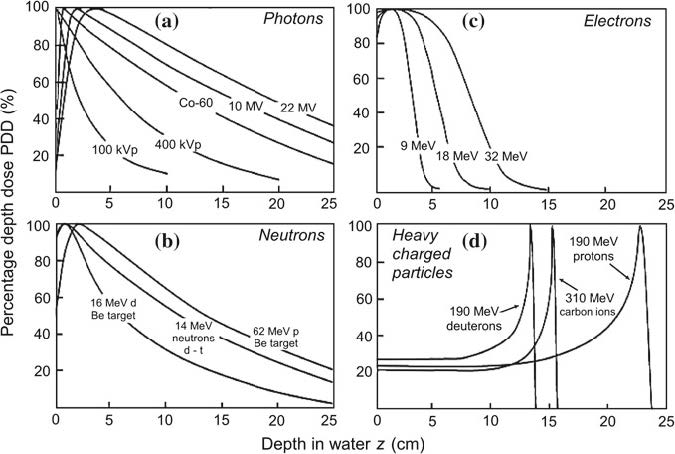
\includegraphics[width=\linewidth]{BraggPeak.jpeg}
            \figcite{Podgorsak2016}
        \end{column}
    \end{columns}
    \note{Schwere geladene Teilchen verlieren Energie nahezu ausschließlich über Kollisionen und bleiben auf einer weitgehend geradlinigen Bahn, bis sie zur Ruhe kommen. Der Bragg-Peak beschreibt den ausgeprägten Anstieg der Energiedepositionsrate am Ende des Teilchenpfades. Während das Teilchen Energie verliert, verlangsamt es sich, und das Bremsvermögen steigt drastisch an \cite[S.\,20]{Podgorsak2016}. Kurz vor dem Stillstand erreicht der Energieverlust pro Weglänge ein Maximum, was die hohe Dosis in einer eng begrenzten Tiefe erklärt.}
\end{frame}

\begin{frame}{Klinische Relevanz}
    \begin{columns}[T,totalwidth=\textwidth]
        \begin{column}{0.52\textwidth}
            \begin{itemize}
                \item Bragg-Peak ermöglicht millimetergenaue Tumordosierung.
                \item Eintrittsdosis geringer, gesundes Gewebe hinter dem Ziel geschont.
                \item Vorteil gegenüber Photonen mit exponentiellem Dosisabfall.
            \end{itemize}
        \end{column}
        \begin{column}{0.45\textwidth}
            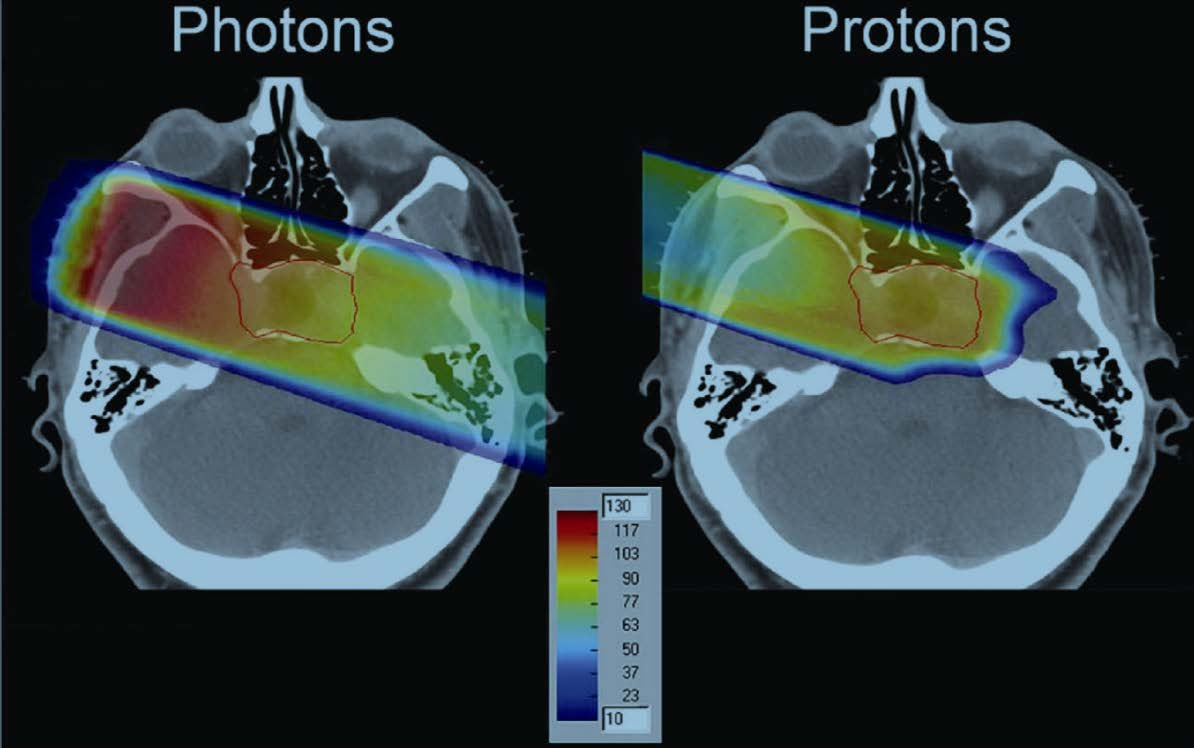
\includegraphics[width=\linewidth]{DSD_88.jpg}
            \figcite{DSD_88}
        \end{column}
    \end{columns}
    \note{Die scharfe Abgrenzung der Dosisdeposition ist der zentrale Vorteil der Hadronentherapie gegenüber der Photonentherapie. Während Photonenstrahlen die Dosis exponentiell verteilen, erlaubt der Bragg-Peak eine millimetergenaue Platzierung der hohen Dosis im Tumor, bei gleichzeitig geringerer Eintrittsdosis und nahezu keiner Dosis hinter dem Zielvolumen \cite{DSD_88}.}
\end{frame}

\begin{frame}{Spread-Out Bragg Peak (SOBP)}
    \begin{columns}[T,totalwidth=\textwidth]
        \begin{column}{0.52\textwidth}
            \begin{itemize}
                \item Monoenergetischer Peak ist zu schmal für klinische Volumina.
                \item Energievariation formt ein Plateau über das Zielvolumen.
                \item Umsetzung über modulierte Abschwächer oder energiegescannte Strahlen.
            \end{itemize}
        \end{column}
        \begin{column}{0.45\textwidth}
            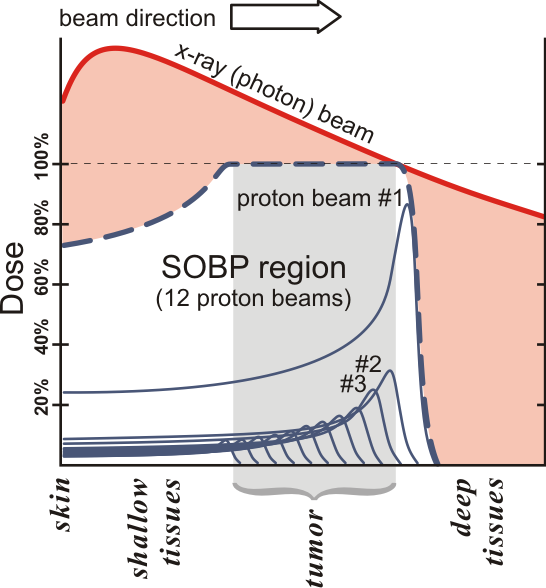
\includegraphics[width=\linewidth]{SOBP.png}
            \figciteweburl{SOBP}
        \end{column}
    \end{columns}
    \note{Der Bragg-Peak eines monoenergetischen Strahls ist sehr schmal. Für größere Tumoren wird ein Spread-Out Bragg Peak erzeugt, indem man Strahlen unterschiedlicher Energie kombiniert. Variable Abschwächer oder energiegescannte Strahlen erzeugen ein Plateau, das der dreidimensionalen Tumorform entspricht \cite{SOBP}.}
\end{frame}

\section{Zusammenfassung}
\begin{frame}{Kerneinsichten}
    \begin{columns}[T,totalwidth=\textwidth]
        \begin{column}{0.58\textwidth}
            \begin{itemize}
                \item Energieverluste teilen sich in Kollisions- und Strahlungsanteile.
                \item Bethe-Formel quantifiziert $S_{\text{col}}$ über Projektile und Material.
                \item Bethe-Kurve erklärt MIP-Minimum und relativistischen Anstieg.
                \item Bragg-Peak ermöglicht präzise Hadronentherapie.
            \end{itemize}
        \end{column}
        \begin{column}{0.37\textwidth}
            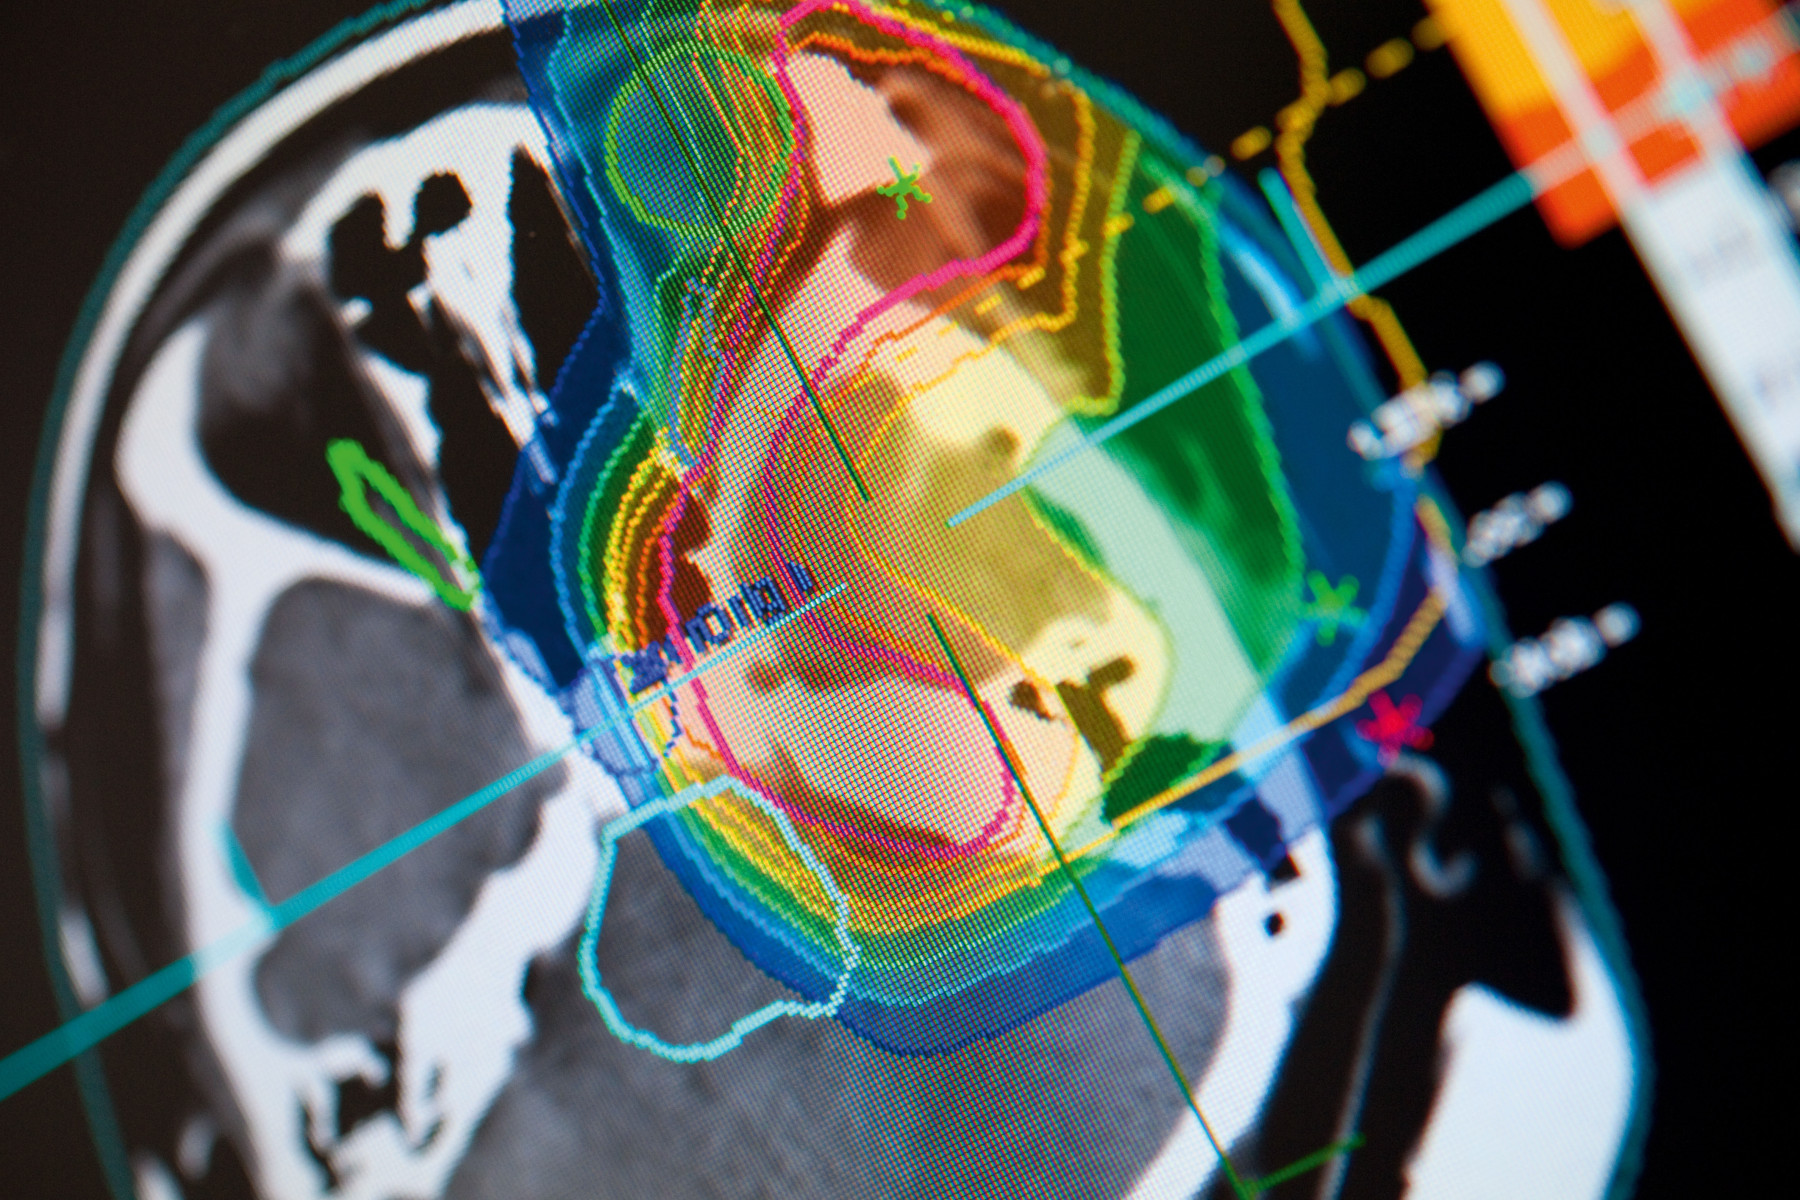
\includegraphics[width=\linewidth]{1920_hirntumorbestrahlung.jpg}
            \figcite{HIT2019Image}
        \end{column}
    \end{columns}
    \note{Wechselwirkungen geladener Teilchen mit Materie lassen sich durch Kollisions- und Strahlungsanteile beschreiben. Das Bremsvermögen quantifiziert die Energierate, wobei für schwere Teilchen die Bethe-Formel den dominierenden Kollisionsanteil liefert und die Material- sowie Geschwindigkeitsabhängigkeit über $1/\beta^{2}$ und $I$ sichtbar macht \cite{Podgorsak2016}. Die Bethe-Kurve zeigt den charakteristischen Verlauf mit MIP-Minimum und relativistischem Anstieg, und die Fähigkeit, den Bragg-Peak zu formen, definiert die moderne Hadronentherapie. Diese Grundlagen sind entscheidend für die präzise Dosimetrie in der Medizinphysik.}
\end{frame}

\begin{frame}[noframenumbering, plain]{Vielen Dank!}
    \vfill
    \centering
    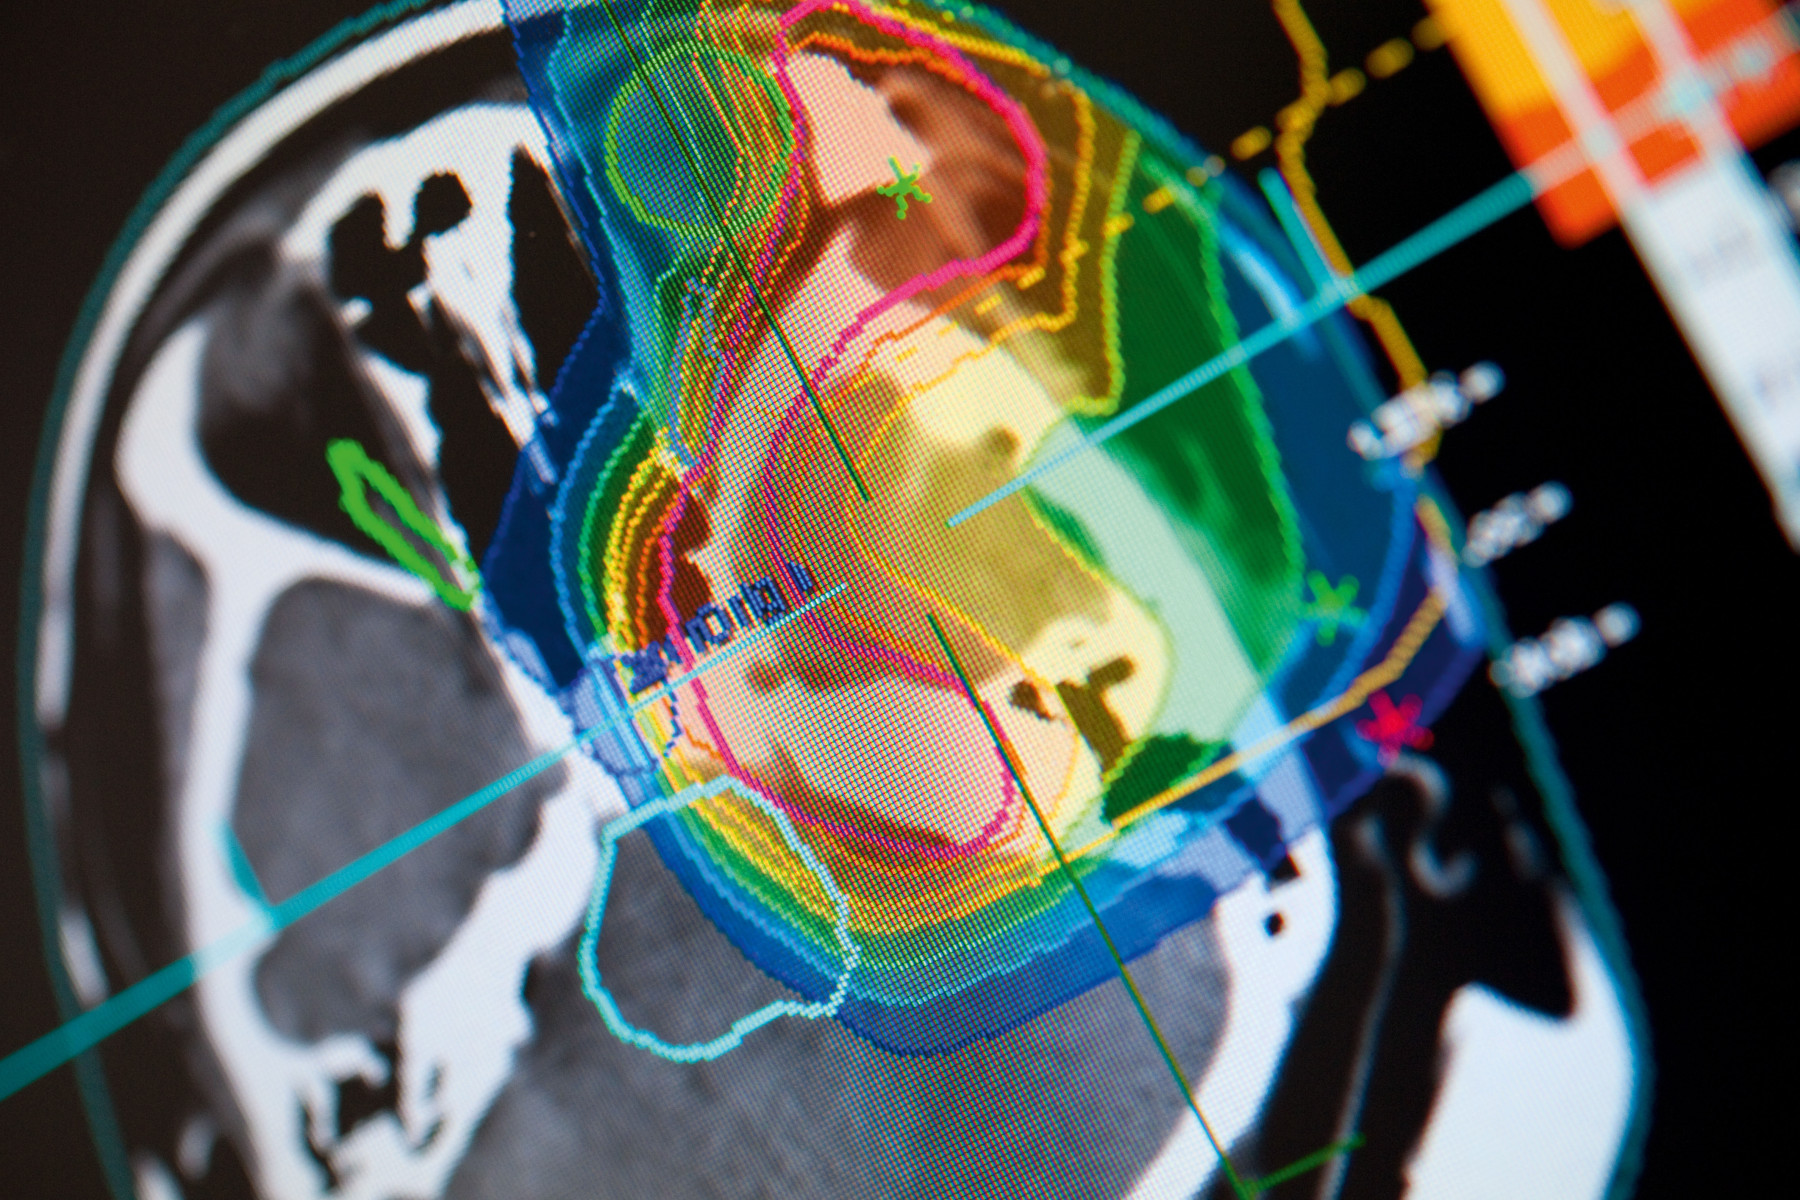
\includegraphics[width=0.8\textwidth]{1920_hirntumorbestrahlung.jpg}
    \figcite{HIT2019Image}
    \vfill
    \note{Ich danke für die Aufmerksamkeit und stehe nun für Fragen zur Verfügung.}
\end{frame}
